% !TEX root = ../../prj4projektdokumentation.tex

\section{Indledning}
I dette afsnit beskrives, hvordan Måleenheden er opbygget. Måleenheden er designet til at kunne måle centralt og decentralt, på projektets simulering af transmissionslinje og forbrugere. Der er på netværket forberedt til at der kan tilsluttes måleenheder på forbrugerne. Spændingen kan måles direkte over forbrugeren. På hver forbruger er der tilsluttet 1 1$\Omega$ modstand i serie. På denne modstand måles spændingen, som vil være proportional med strømmen i systemet. Måleenheden er hovedsageligt software, der sampler og udregninger rms, power factor og THD. Der er dog også lavet hardware til at bearbejde signalerne inden PSOC'en.


\section{Hardware}
\subsection{Indledning}
Måleenhedens hardware skal kunne dæmpe spændingen og forstærke strømmen så det ligger inden for PSOC'ens ADC spændingsområde. ADC kan sample signaler mellem 0 og 5Vpp, Det betyder at signalernes offset skal ændres til 2,5V.

\subsection{Diagram}
På figur \ref{fig:MaalDiagram} ses diagrammet for det hardware der bruges til at dæmpe spændingen, forstærke strømmen og hæve offsettet.

\begin{figure}[H] % (alternativt [H])
	\centering
	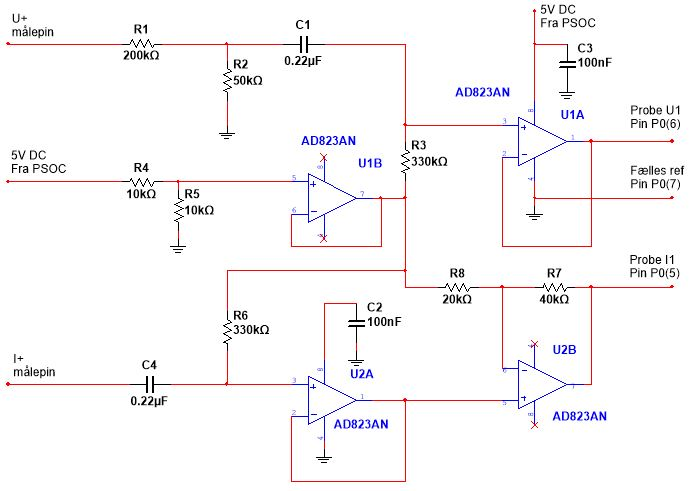
\includegraphics[width=\textwidth]{Figure/MaalHardware}
	\caption{Hardware diagram}
	\label{fig:MaalDiagram}
\end{figure}


\subsubsection{Spændingsmåler}
For at kunne måle den maksimale spænding på 8V rms, dvs.

\begin{align}
Vpp = 8V*\sqrt{2} = 11,3Vpp
\end{align}

Den mindste dæmpning skal derfor være:

\begin{align}
min\_daemp = \dfrac{11.3}{5} = 2,26 gange
\end{align}

Dette er valgt realiseret med en spændingsdeler ved R1 og R2. De dæmper med 3 gange og niveauet kommer derfor indenfor marginen.
Derefter bliver offsettet hævet ved hjælp af signalet fra U1B. Til sidst føres signalet gennem spændingsfølgeren U1A for at sikre spændingen.

\subsubsection{Strømmåling}
Strømmålingen laves ved at måle spændingen over en 1$\Omega$ modstand. Modstanden sidder placeret ved belastningen. Iht. ohmslov vil det give strømmen i systemet
.
\begin{align}
	I = \dfrac{U}{1\Omega} = U
\end{align}

Første Opamp U2A ved strømmålingen bruges til at hæve DC offset til 2,5V. Opamp U2B bruges til at forstærke strømmen så der kommer bedre præcision på målingen. Den maskimale forstærkning, for at den passe indenfor PSOC'ens ADC sample område bliver derfor:

Den maksimale Ipp der vil kunne måles:
\begin{align}
Ipp = 0,5*\sqrt{2} = 0,71A
\end{align}

Maksimale forstærkning:
\begin{align}
maks\_forstaerkning = \dfrac{5}{0,71} = 7
\end{align}
Denne forstærkning ses realiseret vha. modstand R7 og R8.  

\subsubsection{PSOC tilslutning}
Spændingen og strømmen bliver målt til den fælles nul i systemet, der bliver koblet på hardwarens stel forbindelse. Spænding, strøm og stel forbindelsen tilsluttes PSOC'en, som vist på figur \ref{fig:MaalDiagram}.




